\documentclass{article}
\usepackage{graphicx}
\usepackage{xcolor}
\usepackage{amsmath}
\usepackage{amssymb}
\usepackage{authblk}
\usepackage{subcaption}
\usepackage{float}
\usepackage{placeins}
\usepackage{booktabs}
\usepackage{pdflscape}
\usepackage[numbers]{natbib}
\usepackage{setspace}
\usepackage{parskip}
\usepackage{microtype}
\usepackage[margin=2.5cm]{geometry}

\setlength{\parindent}{0pt}
\setlength{\parskip}{7pt}
\linespread{1.15}

\newcommand{\PCAVarI}{39.6\%}
\newcommand{\PCAVarII}{31.1\%}
\newcommand{\PCAVarTotal}{70.6\%}

\title{\textbf{The dynamics live in the loop: route-specific lateral equilibria
of a memoryless controller}}

\author[1]{Peter Ohue}
\author[1]{Emily Oby}
\author[1,2]{Gunnar Blohm}

\affil[1]{Centre for Neuroscience Studies, Queen's University, ON, Canada}
\affil[2]{Department of Biomedical and Molecular Sciences,
          Queen's University, ON, Canada}

\date{}

\begin{document}

\maketitle

%--------------------------------------------------------------
\begin{abstract}
%--------------------------------------------------------------

Unexpected forces can push an ongoing reach toward an obstacle, requiring
the motor system to correct while preserving progress to the target. We
asked whether reward-based learning can produce interpretable population
structure and local stability in a memoryless controller, and whether the
stabilizing dynamics reside in the policy or in its interaction with physics.

We trained a feedforward proximal policy optimization (PPO) actor--critic
for $3\times10^6$ steps to steer a point mass through two obstacles. Its two
256-unit hidden layers received a 13-dimensional observation that included
kinematics, task geometry, heading, and an explicit route cue. We analysed
one hidden layer across 280 episodes (40 per condition, balanced across
left and right routes) in seven conditions: baseline and three lateral-force
magnitudes per direction. Fourteen-step impulses began at step 40.

PCA showed that PC1 and PC2 accounted for 39.6\% and 31.1\% of activity
variance (70.6\% total); trajectories were ordered by movement step and
separated by route, which was explicitly cued. At $y=5$~m, with forward
speed fixed and force removed, the reduced lateral policy--physics loop had
stable, non-oscillatory fixed points at $x^{*}=3.321$~m (left route) and
6.705~m (right), with relaxation times of 1.42~s and 1.34~s. Mean
successful crossing positions were 0.11~m and 0.09~m away. Only the
strongest rightward impulse (1.80) collided: 20/20 left-route episodes;
all other route-by-condition groups succeeded. Because force magnitudes
differed across directions, this does not establish directional
vulnerability. Episode-held-out decoding was 0.11 before and 0.81 after
the impulse (chance 0.143), showing decodability rather than policy use.

Thus, local stabilization resides in the closed policy--environment loop,
not recurrent hidden-state dynamics. This one-seed point-mass model is a
testable computational reference for studying feedback and population
activity in perturbed reaching, not a neural equivalent.

\end{abstract}

%==============================================================
\section{Introduction}
%==============================================================

The ability to reach toward a target while correcting for unexpected
mechanical disturbances is one of the defining capacities of the biological
motor system \citep{Pruszynski2012,Nashed2014,Dimitriou2013,Scott2004}.
When the moving limb is deflected by an external force, the nervous system
does not pause for deliberate decision-making; rapid feedback corrections
emerge within tens of milliseconds, coordinated by the
continuous interplay between sensory inflow and internal predictions about
the limb's future state
\citep{Todorov2002,Todorov2009,Codol2023,FlashHogan1985}.
Critically, this flexibility does not reside in individual neurons.
It emerges from coordinated activity across distributed populations in
motor cortex and cerebellum, populations whose collective dynamics
constitute a low-dimensional trajectory through a high-dimensional
activity space
\citep{Churchland2012,Shenoy2013,Gallego2017,Crevecoeur2019,Blohm2009,Georgopoulos1986,Kalaska1989}.
Understanding how this population-level organisation gives rise to robust,
adaptive behaviour is a central goal of systems motor neuroscience.

Reinforcement learning (RL) offers a complementary computational
perspective on the same problem.
In RL, a controller is not given explicit movement rules; instead, it
discovers a control policy through repeated interaction with an environment,
receiving a scalar reward whenever it performs well and adjusting its
internal parameters accordingly
\citep{Kaelbling1996RLSurvey,SuttonBarto2018,Schulman2017}.
This reward-driven learning is, in spirit, analogous to biological motor
skill acquisition: practice generates sensory and outcome feedback, and the
nervous system gradually refines its internal representation to maximise
successful performance \citep{Oby2019,Mathis2024,Shadmehr1994,WolpertGhahramani2000,Krakauer2019}.
The comparison is not merely metaphorical; both processes involve an agent
updating a policy based on signals about the quality of recent actions,
without being told what the correct movement should have been.

Proximal Policy Optimization (PPO) \citep{Schulman2017}, the algorithm
used here, is a widely adopted policy-gradient method whose update rule is
designed to prevent destabilising changes to the learned policy.
At each training iteration, PPO estimates the relative performance of a
proposed policy update against the current policy and restricts the update
to a bounded neighbourhood around the existing solution, clipping the
probability ratio to the interval $[1-\epsilon, 1+\epsilon]$.
This constraint formalises a principle well-established in motor learning
research: incremental, bounded refinement of the control policy is more
stable than wholesale revision, because large parameter changes risk
degrading performance that has already been acquired \citep{Oby2019,SuttonBarto2018,Heald2021,Krakauer2019}.
The term ``proximal'' refers precisely to this neighbourhood constraint:
updates stay close to the current policy, producing steady improvement
without the catastrophic performance swings that unconstrained gradient
ascent can generate.

Despite strong task performance, most RL studies evaluate controllers
solely on behavioural outcomes such as success rate, cumulative reward,
and mean path length, treating the policy network as a black box
\citep{Rudin2019,Molnar2022}.
This characterisation is informative but mechanistically incomplete: it
cannot explain which internal signals distinguish a trial in which the
agent successfully corrects from one that ends in collision.
Identifying such signals is precisely the kind of question that
population-level analyses have addressed in biological motor cortex
\citep{Churchland2012,Cunningham2014,Gallego2017,Blohm2009}.

Population activity in motor cortex during reaching evolves along smooth,
low-dimensional neural manifolds, defined as compact subspaces within the
high-dimensional activity space that capture the essential structure of
movement generation
\citep{Churchland2012,Shenoy2013,Cunningham2014,Gallego2017,Sadtler2014,Elsayed2016,Kaufman2014}.
Individual neurons within these populations exhibit heterogeneous tuning
to kinematic variables, but the population as a whole encodes these
variables in a structured, often linearly readable form
\citep{Oby2019,Blohm2009,Georgopoulos1986,Perich2018}.
These observations motivate the central question of this study: does an
artificially trained controller that was never designed to resemble a
biological motor system develop similar representational organisation as a
natural consequence of reward-driven learning?

We trained a PPO controller on a two-dimensional obstacle-avoidance reaching
task and evaluated it under seven lateral-force conditions, with left- and
right-route cues balanced across episodes. At each timestep we extracted
activity from one hidden layer and analysed it as an artificial
population-state vector, not as a biological recording. We used PCA,
clustering, kinematic tuning, and episode-held-out linear decoding to
characterise its relation to movement and perturbation condition. We then
analysed the policy coupled to the physics engine to ask whether local
stability can be identified in the reduced lateral dynamics.

The central result is a distinction between the feedforward policy and its
closed loop: the hidden layer has no autonomous temporal dynamics, whereas
the policy--environment system has route-specific, locally stable lateral
fixed points when forward position and speed are held fixed. This
complements population-state analyses with a physical-state account of local
stabilization. Route separation in the activity must be interpreted in light
of an explicit route cue in the policy observation, and the single-seed,
point-mass design limits biological inference.


%==============================================================
\section{Methodology}
%==============================================================

\subsection{Task Environment}

We implemented the obstacle-avoidance environment using the Gymnasium
interface \citep{Towers2024Gymnasium}, a standard open-source framework
for defining physics-based reinforcement learning environments.
The agent is a two-dimensional point mass that receives continuous force
commands at each timestep and evolves under Newtonian dynamics within a
bounded rectangular workspace.
We deliberately kept the dynamics minimal (a single point mass with no
rotational degrees of freedom and no joint limits) so that any
representational structure found in the trained network is attributable
to learning rather than to the complexity of the physical system.
This minimalism also makes the setup directly comparable to the planar
arm-perturbation paradigms used in human motor neuroscience, where the
task geometry rather than the limb dynamics is the primary independent
variable \citep{Nashed2014,Pruszynski2012,Shadmehr1994,Franklin2011}.

Figure~\ref{fig:schematic} illustrates the task and analysis pipeline.
Panel~A uses a planar arm and brain schematic to connect the setup to the
biological literature; all experiments use the point-mass dynamics
summarized in Panel~C.
Panel~B shows the PPO actor--critic loop that governs learning.

\begin{figure}[H]
  \centering
  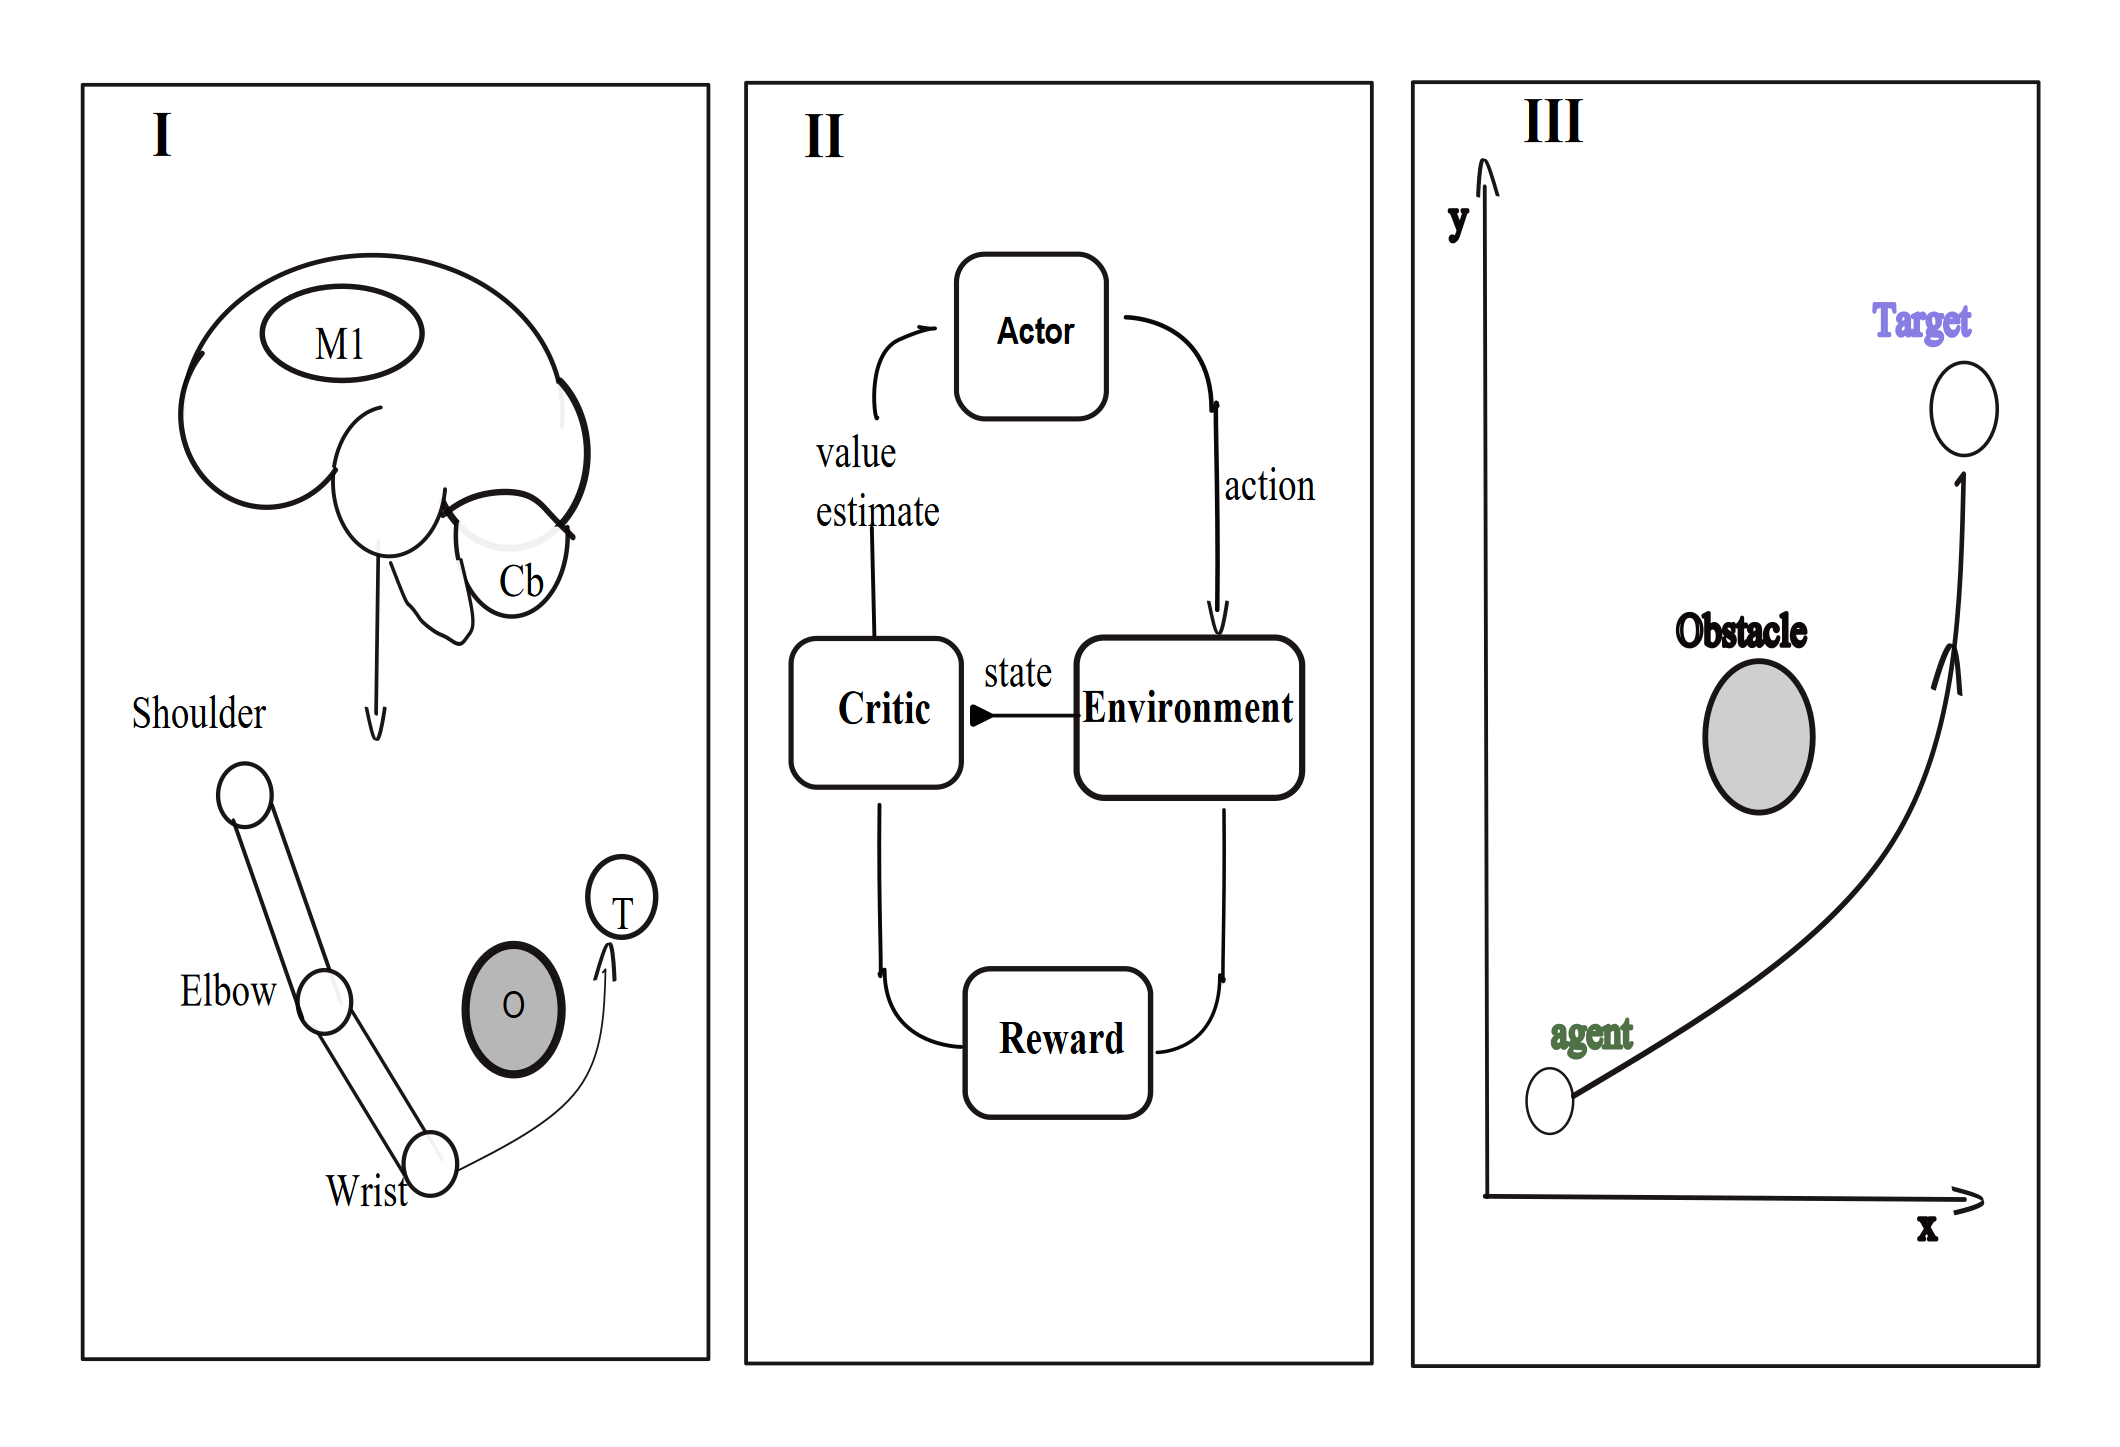
\includegraphics[width=0.88\linewidth]{fig1_schematic.png}
  \caption{\textbf{Task design, control architecture, and population
    analysis pipeline.}
    \textbf{(A)}~Biological analogy illustrating the conceptual parallel
    between the artificial controller and biological motor control.
    Primary motor cortex (M1) provides descending drive to the shoulder,
    elbow, and wrist, guided by cerebellar (Cb) predictions and sensory
    feedback, to move a multi-joint arm toward a target~(T) while avoiding
    an obstacle~(O). This panel situates the computational setup in the
    language of systems motor neuroscience; the actual experiments use a
    point-mass agent.
    \textbf{(B)}~The PPO actor--critic control loop. At each timestep,
    the \emph{actor} network receives the current state observation and
    outputs a continuous force command (the action). The
    \emph{environment} applies that command, advances the agent one
    timestep, and returns the new state. The \emph{critic} network
    receives the state and estimates its long-term value; together with the
    observed reward, this estimate is used to compute the advantage that
    guides the actor's update. A scalar reward signal is produced
    by the environment at every timestep to drive both networks.
    \textbf{(C)}~Task geometry. The agent (green dot) starts at a fixed
    position at the bottom of the workspace and must navigate to a fixed
    goal (top) on a two-dimensional Cartesian plane, while avoiding
    the obstacle(s) in the corridor between start and goal.}
  \label{fig:schematic}
\end{figure}

The main perturbation experiment used a corridor formed by two static
circular obstacles positioned symmetrically about the midline of the
workspace.
The corridor is narrow enough that trajectories deflected by strong lateral
perturbations risk collision with one of the obstacle boundaries, making
it a sensitive test of online correction ability.
A preliminary single-obstacle experiment was run first to establish the
basic obstacle-avoidance skill; the two-obstacle configuration was then
introduced and training continued until performance plateaued.

\subsection{State Representation}

The agent's observation at each timestep combines physical state, task
geometry, and the desired route cue:
\begin{equation}
  s_t = \bigl[
    x_t,\;y_t,\;v_{x,t},\;v_{y,t},\;
    g_x - x_t,\;g_y - y_t,\;
    o_{Lx} - x_t,\;o_{Ly} - y_t,\;
    o_{Rx} - x_t,\;o_{Ry} - y_t,\;
    d_{g,t},\;\theta_t,\;r_t
  \bigr]
  \label{eq:state}
\end{equation}
where $(x_t,y_t)$ and $(v_{x,t},v_{y,t})$ are position and velocity,
$(g_x,g_y)$ is the target-relative coordinate pair, $(o_L,o_R)$ are the
obstacle centres, $d_{g,t}$ is distance to target, $\theta_t$ is heading,
and $r_t\in\{-1,+1\}$ specifies the left or right detour. The observation
is 13-dimensional. Because route identity is provided explicitly,
separation of routes in hidden activity is not evidence that the policy
inferred route identity from sensory input alone.

\subsection{Reward Function}

The agent receives a scalar reward at each timestep that encodes four
distinct objectives:
\begin{equation}
  R_t = w_p\,\Delta d_{\mathrm{goal}}
        - w_v\,\|v_t\|
        - w_c\,C_t
        + w_s\,S_t
  \label{eq:reward}
\end{equation}
The first term rewards reduction in the Euclidean distance to the goal
($\Delta d_{\mathrm{goal}} > 0$ when the agent moves closer);
the second penalises excessive instantaneous speed to encourage smooth
movements;
the third imposes a large negative penalty upon collision with an obstacle
($C_t = 1$ at collision, $0$ otherwise);
and the fourth provides a terminal bonus upon successful goal attainment
($S_t = 1$ at success, $0$ otherwise).
The weights $w_p, w_v, w_c, w_s$ were tuned so that efficient goal-seeking
was the dominant objective while collision avoidance remained a hard
constraint in practice.

\subsection{Perturbation Protocol}
\label{sec:methods-perturbation}

To probe the controller's capacity for online correction, we applied
transient lateral force impulses mid-movement during evaluation.
The impulse magnitude was held constant for fourteen consecutive timesteps
beginning at timestep 40:
\begin{equation}
  f_x(t) = p_i + \epsilon_t, \quad t \in [40,\,53], \quad
  \epsilon_t \sim \mathcal{N}(0,\,0.05^2)
  \label{eq:perturbation}
\end{equation}
A positive value of $p_i$ corresponds to a rightward impulse; a negative
value to a leftward impulse.
This yields seven evaluation conditions: an unperturbed control (P0) and
three increasing leftward perturbations (L1: $-0.40$, L2: $-0.60$, L3:
$-0.85$) and three increasing rightward perturbations (R1: $+0.40$, R2:
$+0.65$, R3: $+1.80$).
The magnitudes are not evenly spaced.
R3 is more than twice the size of L3.
All analyses of the representations and of the closed loop use one set of
rollouts: the checkpoint saved as \texttt{best\_model}, 40 episodes per
condition, alternating between the left and right route cue, with a
fixed random seed.
The agent's forward speed is capped at 1.0, and episodes last about
160--170 timesteps.
The fourteen-timestep window is brief relative to that duration, mimicking the short-duration
mechanical perturbations applied in biological reaching paradigms to
isolate online feedback responses from anticipatory motor planning
\citep{Pruszynski2012,Nashed2014,Dimitriou2013,Todorov2002,Shadmehr1994}.

\subsection{Reinforcement Learning Controller and Training}

All training and evaluation used Stable-Baselines3
\citep{Raffin2021StableBaselines3}, an open-source Python library built
on PyTorch that provides rigorously tested implementations of standard
deep RL algorithms.
We used Proximal Policy Optimization (PPO) \citep{Schulman2017}, which
maximises the following clipped surrogate objective:
\begin{equation}
  L^{\mathrm{CLIP}}(\theta) = \mathbb{E}_t\!\Bigl[
    \min\!\bigl(r_t(\theta)\hat{A}_t,\;
    \mathrm{clip}(r_t(\theta),1-\epsilon,1+\epsilon)\hat{A}_t\bigr)
  \Bigr]
  \label{eq:ppo}
\end{equation}
Here $r_t(\theta) = \pi_\theta(a_t|s_t) / \pi_{\theta_{\mathrm{old}}}(a_t|s_t)$
is the probability ratio of the new policy to the old policy,
$\hat{A}_t$ is the generalized advantage estimate (a measure of how much
better the selected action was relative to the expected value of that
state), and $\epsilon = 0.2$ is the clipping parameter that restricts
the policy ratio to the interval $[1-\epsilon, 1+\epsilon]$, bounding
the size of any single update step.

The policy and value networks are separate feedforward multilayer
perceptrons (MLPs), each with two hidden layers of 256 units and
rectified linear (ReLU) activations.
A feedforward MLP processes each timestep independently, without recurrence
or explicit memory of previous states.
Continuous actions are drawn from a diagonal Gaussian distribution whose
mean is output by the actor network; the standard deviation is a learned
parameter.
Observations were standardised online using a running mean and variance
(VecNormalize), which substantially improves training stability in
continuous-control settings.
Training ran for $3\times10^6$ environment timesteps with the following
hyperparameters: learning rate $\alpha = 3\times10^{-4}$, discount factor
$\gamma = 0.99$, generalised advantage estimation parameter
$\lambda_{\mathrm{GAE}} = 0.95$, entropy regularisation coefficient
$c_{\mathrm{ent}} = 0.005$, value-function loss coefficient $c_v = 0.5$,
and maximum gradient norm $0.5$.
All experiments were run with Stable-Baselines3 v2.8.0, Gymnasium,
and PyTorch on an Intel\textregistered\ Core\textsuperscript{TM} Ultra~7~255H
processor.

\subsection{Neural Population Analysis Pipeline}

Following training convergence, we extracted the activation vector
$h_t \in \mathbb{R}^{256}$ from the first hidden layer of the policy
network at every timestep $t$ of every evaluation episode.
Let $T$ denote the length of an episode; the full population record for
that episode is:
\begin{equation}
  H = \{h_1, h_2, \ldots, h_T\}
  \label{eq:latent}
\end{equation}
Concatenating $H$ across all evaluation episodes gives a matrix of
shape $N_{\mathrm{total}} \times 256$, where $N_{\mathrm{total}}$ is the
total number of timesteps across all episodes and conditions.

Three population-level analyses were then applied to this matrix.

\textbf{Principal Component Analysis (PCA).}
PCA finds a set of orthogonal directions, called principal components, that
account for successively decreasing fractions of the total variance in
the population data.
Projecting the 256-dimensional activity onto the first two principal
components provides a two-dimensional visualisation of the population
state space and allows us to quantify how compactly the activity is
organised.
We report the fraction of total variance explained by each principal
component as a direct measure of dimensionality compression.

\textbf{Kinematic tuning analysis.}
For each of the 256 hidden units, we computed the Pearson correlation
between its activation and instantaneous lateral velocity across all
evaluation timesteps.
This identifies units that are systematically modulated by the direction
or magnitude of lateral movement, analogous to single-unit tuning analyses
in biological motor electrophysiology.

\textbf{Linear decoding.}
We trained a multinomial logistic regression classifier (regularisation
$C = 1.0$) on single-timestep hidden-layer activity to predict which of
the seven perturbation conditions was active.
A linear classifier was used deliberately: if strong decoding performance
can be achieved with a linear readout, it implies that the relevant
information is encoded in the geometry of the population activity in a
relatively direct, structured way rather than requiring nonlinear
transformations to extract.
Classifier performance is summarised as a confusion matrix across
conditions.
All analyses were implemented in Python using NumPy, SciPy, and
scikit-learn.

\subsection{Dynamical-Systems Framework for the Closed Loop}
\label{sec:dynsys}

PCA, clustering, and decoding describe hidden-activity geometry; they do
not identify the physical dynamics that stabilize movement. The actor is
feedforward, so its hidden activity is a static function of the current
observation rather than a recurrent state. We therefore analysed the
policy coupled to the physics engine. The full system advances through the
corridor and has no stationary fixed point during a reach. For local
stability analysis, we held forward position and speed fixed, removed the
external force, and analysed the reduced lateral map
$(x,v_x)\mapsto(x_{t+1},v_{x,t+1})$ separately for each route cue. The
equilibria reported below are fixed points of this reduced map at a
specified forward position, not fixed points of the hidden layer or of the
full moving reach.

\textbf{State, trajectory, vector field.}
A dynamical system is a rule for how a state changes over time. Here the
policy and physics together map the agent's current observation and
physical state to a new physical state. The complete reach remains in
motion, so it is not stationary. To examine local lateral stability, we
fixed forward position $y$ and forward speed at their cruising value,
specified the route cue, and considered the impulse-free lateral dynamics.
This defines a reduced two-dimensional map over lateral position $x$ and
lateral velocity $v_x$. A trajectory through the actual task is not
identical to a trajectory of this reduced map; the latter isolates local
lateral correction at one forward position.

\textbf{Fixed points, stability, attractors.}
A \emph{lateral fixed point} is a state unchanged by the reduced map:
lateral velocity is zero and the commanded lateral acceleration is zero,
while forward position, forward speed, and route cue are held fixed.
Whether a fixed point matters behaviourally depends on its
\emph{stability}. Perturbing the state slightly and linearising the
vector field around the fixed point yields a matrix, the \emph{Jacobian},
whose eigenvalues describe what happens next. In discrete time (the
simulation advances in fixed steps of $dt=0.05$~s), an eigenvalue with
magnitude below 1 means that direction decays back to the fixed point, an
\emph{attractor} along that direction; magnitude above 1 means it grows
away, a \emph{repeller}; a nonzero imaginary part means the decay
oscillates on the way back in rather than returning in a straight line. A
fixed point's \emph{basin of attraction} is the set of starting lateral
states that approach it under the same clamped forward position, speed,
and route cue. These local equilibria should not be interpreted as
stationary attractors of the entire forward-moving trajectory.

\textbf{Why a feedforward policy still has a closed loop.}
The classic version of this analysis (Sussillo and Barak, 2013) finds
fixed points of a recurrent network's own hidden state, because a
recurrent unit's activity at time $t+1$ is a function of its activity at
time $t$. Our policy is feedforward: the 256-unit hidden layer analysed
in Figure~\ref{fig:pca} is a static function of the instantaneous
observation, $h_t = g(s_t)$, with no memory of its own previous value, so
``the fixed points of the hidden layer'' is not a well-posed question
here. What \emph{is} well posed, and what we compute instead, is the
fixed points of the policy--environment loop in the reduced lateral
physical state space. This analysis uses fixed forward position and speed;
it is not a substitute for fixed-point analysis of a recurrent network and
does not imply that this feedforward actor has hidden-state dynamics.

%==============================================================
\section{Results}
%==============================================================

We evaluated the trained PPO controller across all seven perturbation
conditions (P0, L1--L3, R1--R3) and report findings in four parts,
proceeding from observable behaviour to the internal representations that
underlie it.

Figure~\ref{fig:trajectories} shows the 280 evaluation trajectories: 40 per
condition, balanced across the two route cues. The controller reached the
goal in every route-by-condition group except R3 on the left route, where
all 20 episodes collided. The corresponding 20 R3 episodes on the right
route succeeded. All 20 episodes succeeded in each of the other six
conditions on both routes. Thus, the observed failure is specific to the
strongest tested rightward impulse on the left route; because leftward and
rightward force magnitudes were not matched, these data do not establish a
general directional asymmetry.

\begin{figure}[H]
  \centering
  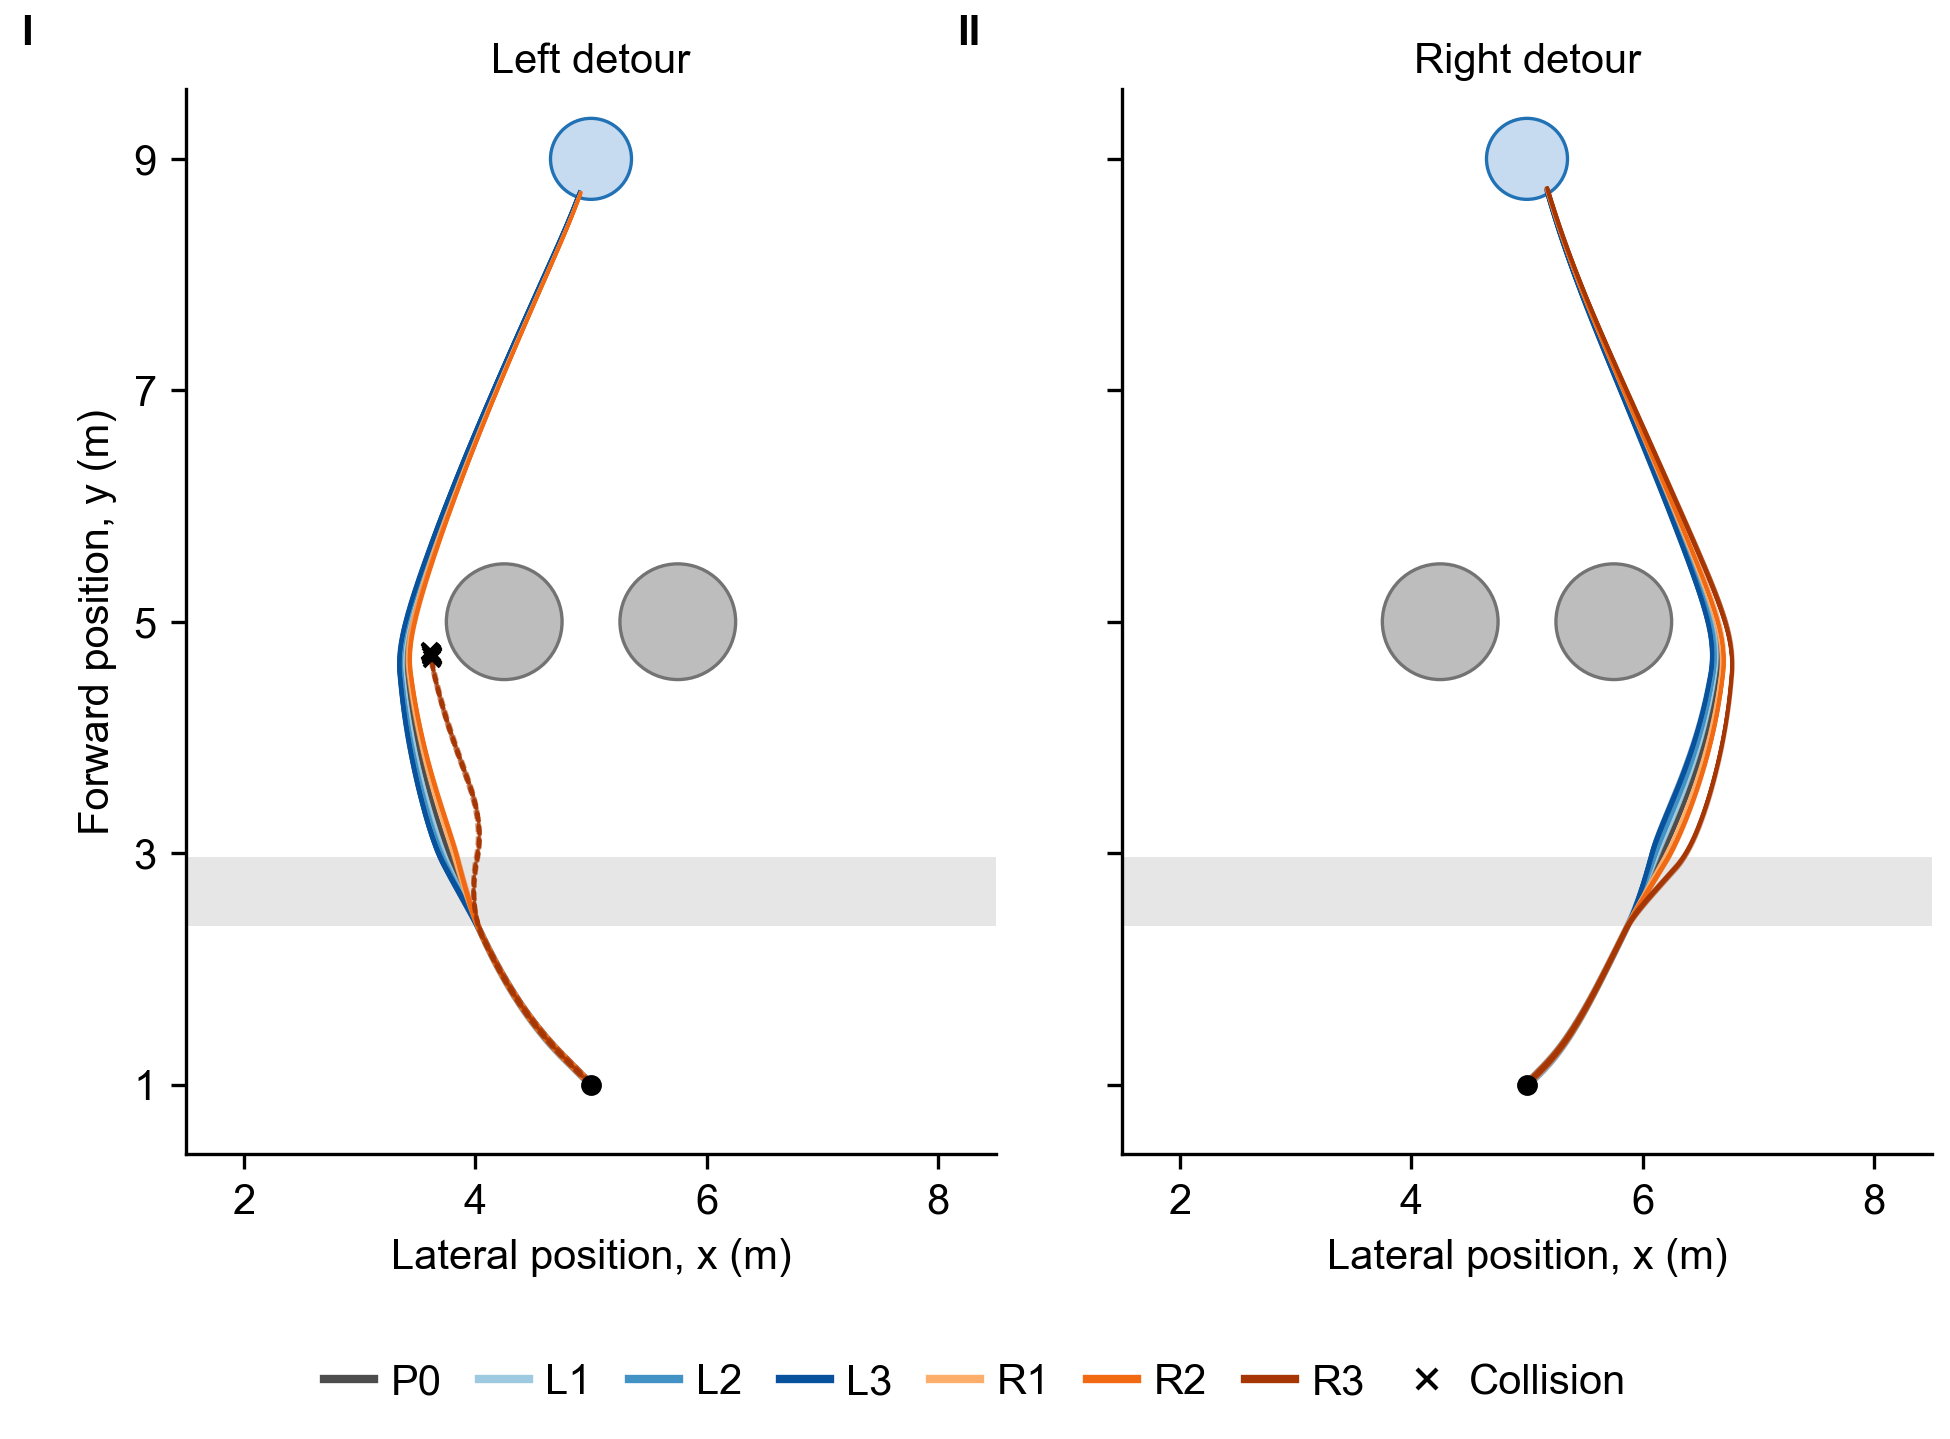
\includegraphics[width=0.58\linewidth]{fig2_trajectories.png}
  \caption{\textbf{Reach trajectories across the seven perturbation
    conditions and two route cues.}
    Each evaluation episode is overlaid separately for each condition and
    route cue (20 episodes per route and condition).
    Solid lines are successful trials that reached the goal; the dashed
    red lines are failure trajectories that ended in obstacle collision.
    Leftward perturbation conditions (L1--L3, mauve/pink tones) progressively
    deflect the path toward the left obstacle, while rightward conditions
    (R1--R3, teal/dark green) deflect it toward the right.
    The shaded band marks the workspace region corresponding to the
    14-step impulse beginning at step 40.
    Grey ellipses represent the two static obstacles forming the corridor.
    All route-by-condition groups succeeded in 20/20 episodes except the
    strongest rightward condition (R3) on the left route, which collided in
    20/20 episodes. R3 succeeded in 20/20 episodes on the right route.}
  \label{fig:trajectories}
\end{figure}

The data establish robustness across the tested conditions and routes, with
one specific failure group. The left- and rightward force magnitudes are
unequal, however, so comparing their outcomes cannot isolate a causal
effect of perturbation direction or obstacle clearance.

Figure~\ref{fig:velocity} characterises the temporal evolution of
lateral velocity and total speed across all seven conditions.

\begin{figure}[H]
  \centering
  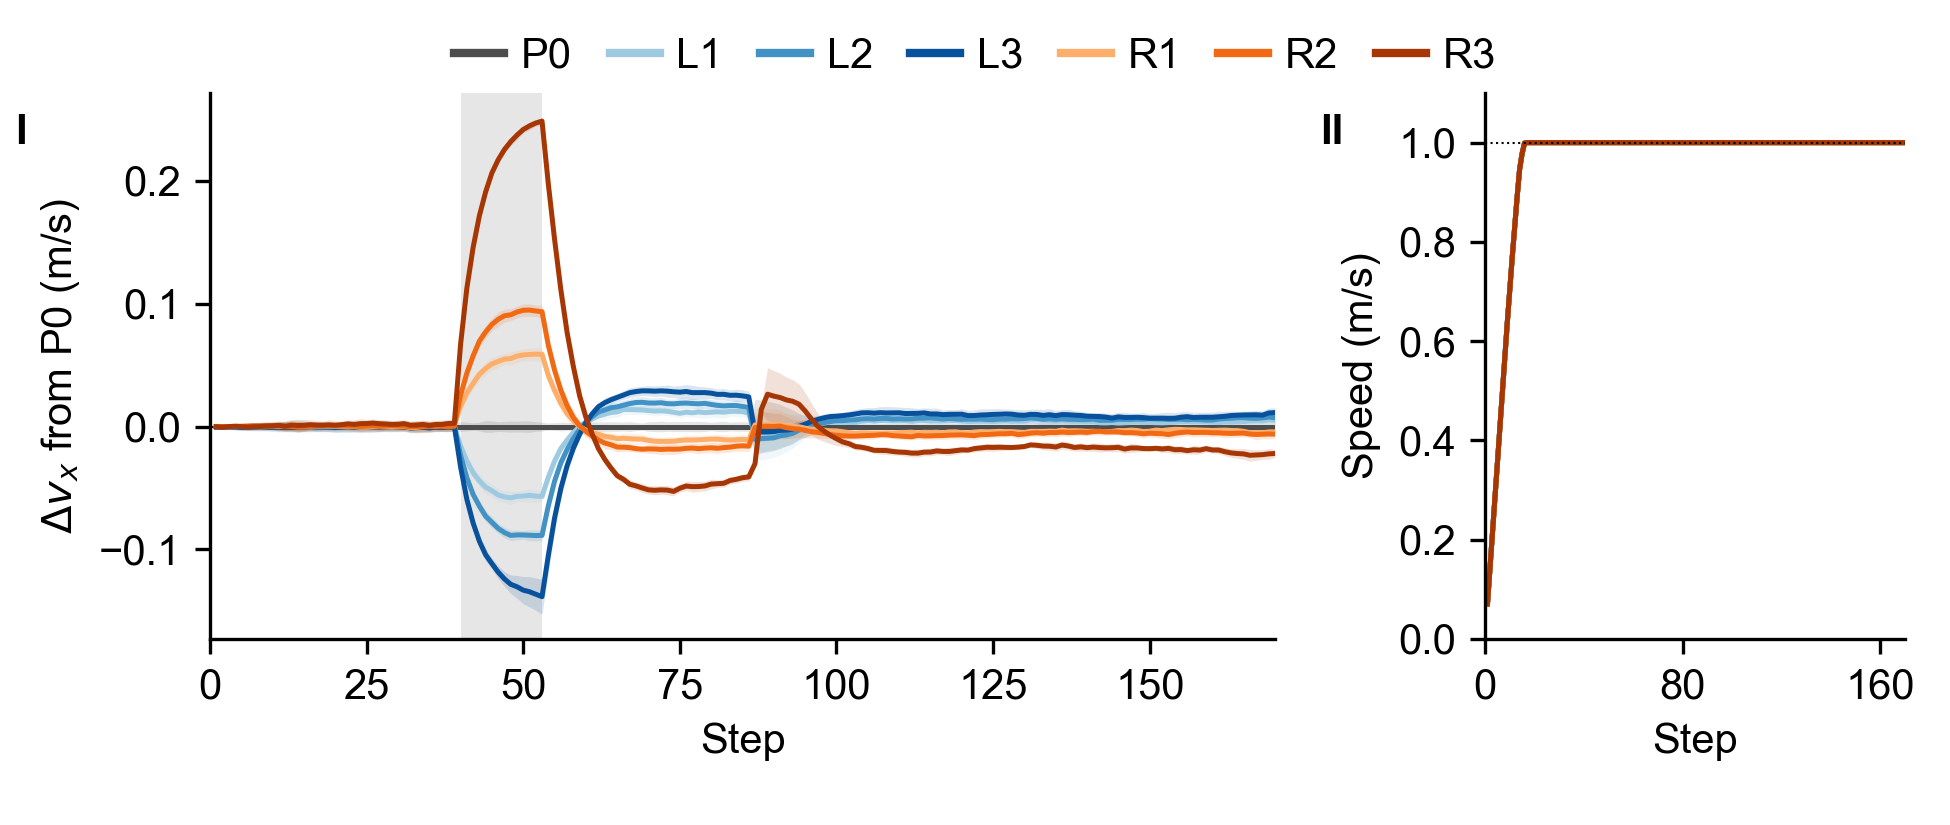
\includegraphics[width=0.80\linewidth]{fig3_velocity.png}
  \caption{\textbf{Lateral velocity and speed profiles during
    perturbation.}
    \textbf{(I)}~Mean lateral velocity, expressed as a deviation from the
    unperturbed (P0) trajectory ($\Delta v_x$), over time, aligned to
    movement onset and averaged across all episodes within each condition.
    Shaded regions show $\pm$1\,SD, conveying trial-to-trial variability.
    We plot the deviation from P0 rather than raw lateral velocity because
    route is accounted for when comparing perturbed and unperturbed
    trajectories; subtracting the baseline isolates the perturbation
    response from the route-specific movement pattern.
    Leftward conditions (L1--L3) push $\Delta v_x$ negative, while
    rightward conditions (R1--R3) push it positive during the perturbation
    window (steps 40--53, indicated by the shaded band).
    After the impulse, lateral velocity returns toward the corresponding
    route-specific baseline. These profiles describe the kinematic response
    and do not by themselves establish a proportional feedback law.
    \textbf{(II)}~Total speed (Euclidean norm of the velocity vector)
    plotted as a function of normalised movement phase (0 = movement onset,
    100 = goal arrival). Shading shows trial-to-trial variability.}
  \label{fig:velocity}
\end{figure}

Panel~I shows the change in lateral velocity relative to the unperturbed
trajectory during and after the impulse. This describes the kinematic
response in the simulated task; it does not by itself identify a
biological feedback mechanism. Panel~II shows total speed over movement
phase. We use these profiles descriptively and do not infer a general
separation between lateral correction and movement tempo from this
single-seed evaluation.

Figure~\ref{fig:pca} shows the result of projecting the full 256-dimensional
hidden-layer activity onto its first two principal components across all
evaluation timesteps.

\begin{figure}[H]
  \centering
  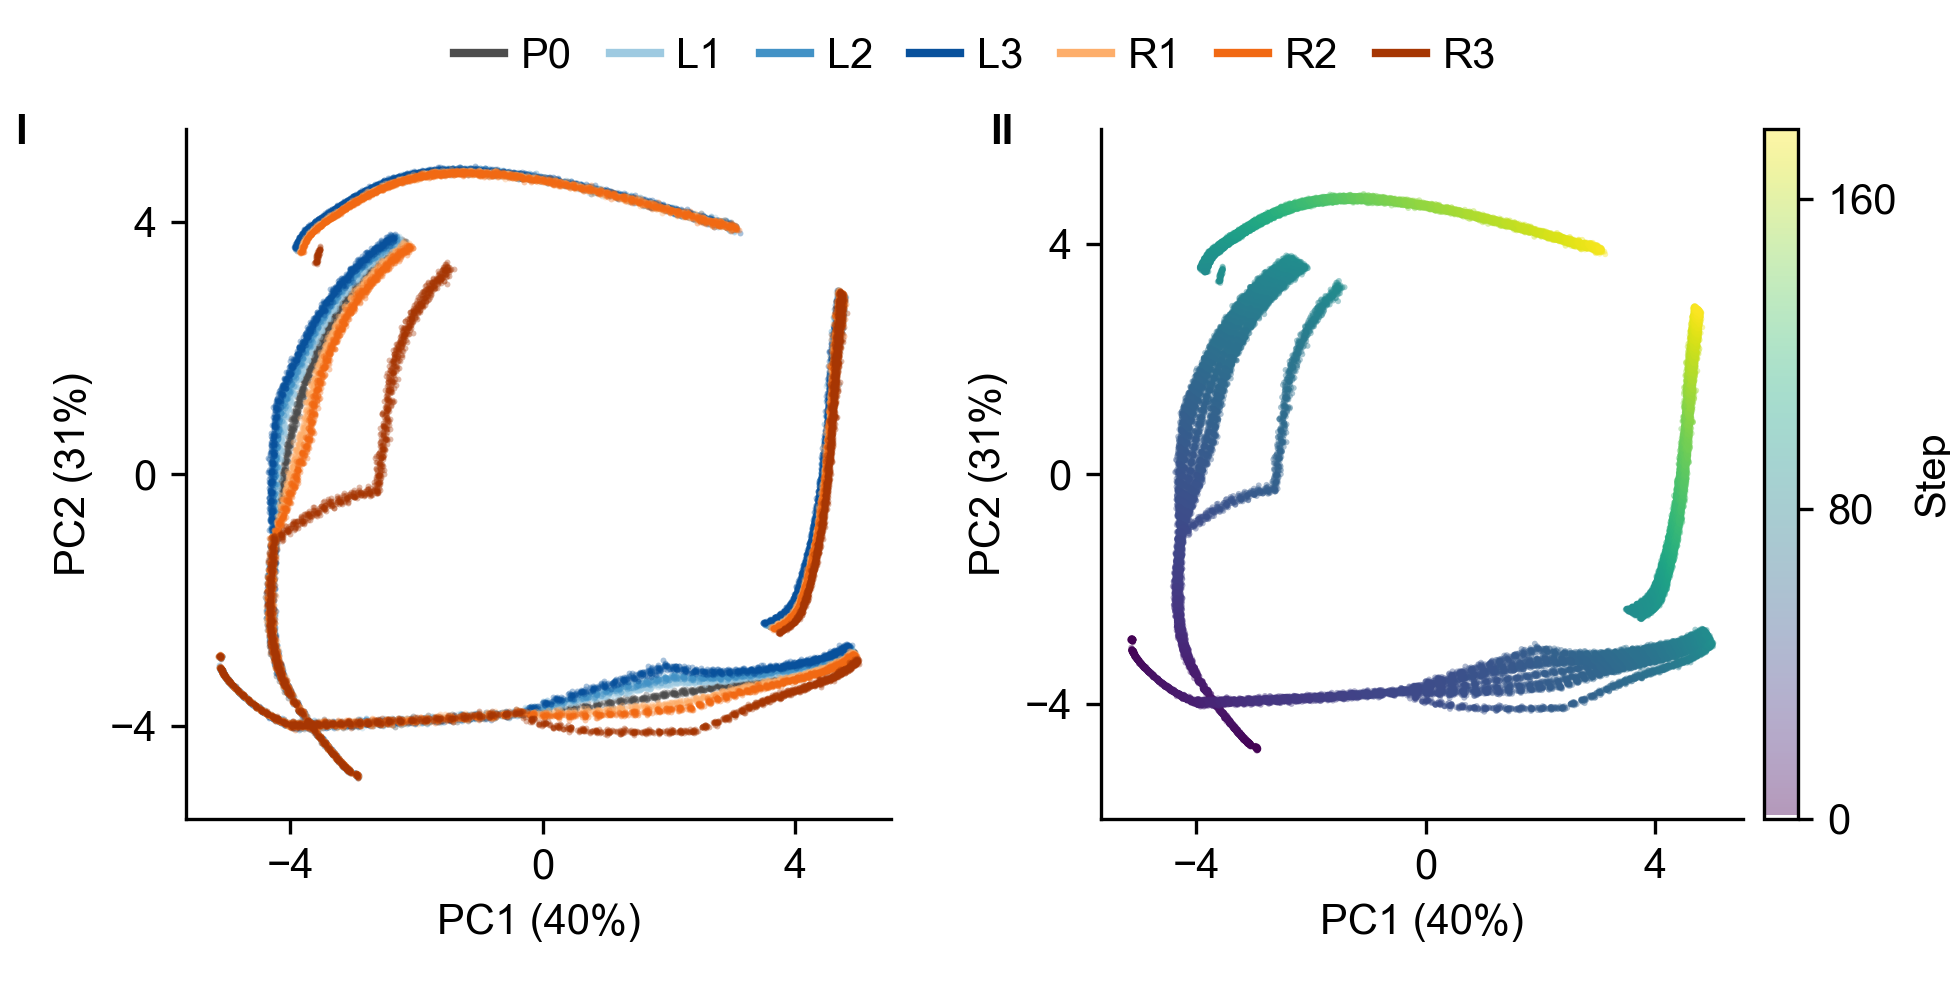
\includegraphics[width=0.88\linewidth]{fig4_pca.png}
  \caption{\textbf{Hidden-layer activity occupies a low-dimensional
    manifold ordered by movement phase.}
    Each point represents the 256-dimensional hidden-state vector at one
    timestep of the rollouts, projected onto the first two principal
    components of the full rollout set (40 episodes per condition).
    \textbf{(I)}~Points are coloured by perturbation condition. Activity
    separates by detour route; the route cue is an explicit component of the
    policy observation. Within each route, trajectories show condition-
    dependent variation after the impulse.
    PC1 accounts for \PCAVarI{} of the variance and PC2 for \PCAVarII{},
    \PCAVarTotal{} in total.
    \textbf{(II)}~The same projection coloured by step. Activity moves
    along each branch from the start (dark) to the goal (light).}
  \label{fig:pca}
\end{figure}

Two principal components account for \PCAVarTotal{} of the variance in the
analysed 256-unit layer (PC1: \PCAVarI{}; PC2: \PCAVarII{}). This is a
compact description of activity in these rollouts, but it does not establish
that the network learned a biological-style neural manifold. The task
repeatedly samples a restricted set of movement states, and route is
explicitly specified in the observation; both factors can contribute to the
observed geometry. Low-dimensional population structure is also reported in
motor-cortical reaching data
\citep{Churchland2012,Shenoy2013,Cunningham2014,Gallego2017,Sadtler2014,Elsayed2016},
providing a useful organizational comparison rather than evidence of
equivalent mechanisms.

Activity also varied systematically with route and movement step. The route
cue was perfectly decodable (held-out accuracy 1.00; chance 0.50), as
expected for an explicit input. Exploratory $K$-means clustering ($K=4$)
within each route produced clusters ordered over movement time. Their
condition composition was broadly similar, although later clusters on the
left route were affected by early termination of R3 collisions. The choice
of $K$ was not cross-validated, and clustering was not repeated across
training seeds. We therefore treat this phase ordering as descriptive,
not as evidence for discrete biological population states
\citep{Churchland2012,Shenoy2013,Kaufman2014,Perich2018}.

Figure~\ref{fig:decoding} shows the confusion matrix from a linear
classifier trained on single-timestep hidden-layer activity to identify
the perturbation condition active on each trial.

\begin{figure}[H]
  \centering
  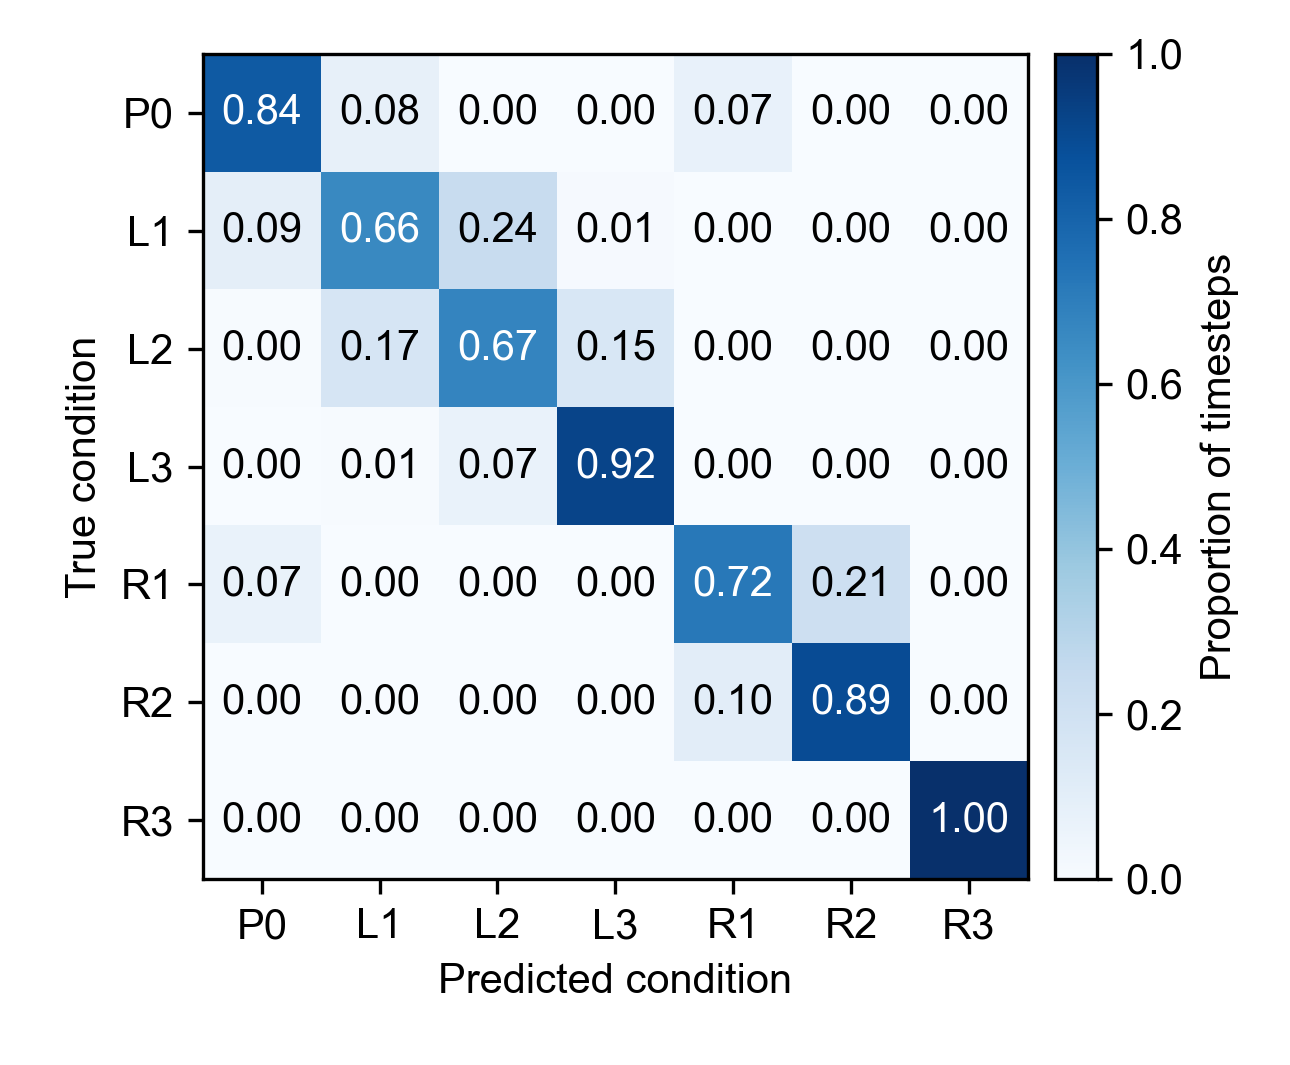
\includegraphics[width=0.56\linewidth]{fig5_decoding.png}
  \caption{\textbf{A linear decoder identifies the perturbation condition
    after the impulse, not before it.}
    Rows are the true condition and columns the condition predicted by a
    multinomial logistic regression on the 256-dimensional hidden-layer
    vector at one timestep. Entries are row-normalised.
    Accuracy was estimated with five-fold episode-held-out
    cross-validation. The matrix shows timesteps after the impulse
    (steps 54--100, accuracy 0.81, seven-class chance 0.143).
    Before the impulse (steps 0--39), accuracy was 0.11, near chance.
    Errors fall mostly between neighbouring magnitudes on the same side
    (L1 as L2, R1 as R2).}
  \label{fig:decoding}
\end{figure}

In episode-held-out cross-validation, perturbation condition was decoded at
0.11 accuracy before the impulse and 0.81 after it (chance 0.143 for seven
classes). This establishes that condition-related information is linearly
readable from the activity after the impulse. It does not show that the
policy uses this information to select its action. Because the actor is
memoryless and its observation contains current kinematics and task context,
the decoder may be reading state changes caused by the impulse rather than
a stored representation of perturbation history. Linear decoding is used
in motor-cortical population analyses as well
\citep{Churchland2012,Nashed2014,Oby2019,Georgopoulos1986,Sadtler2014};
the interpretation here is limited to this controller and task.

Figure~\ref{fig:learning} contextualises the representational findings
within the training dynamics of the controller.

\begin{figure}[H]
  \centering
  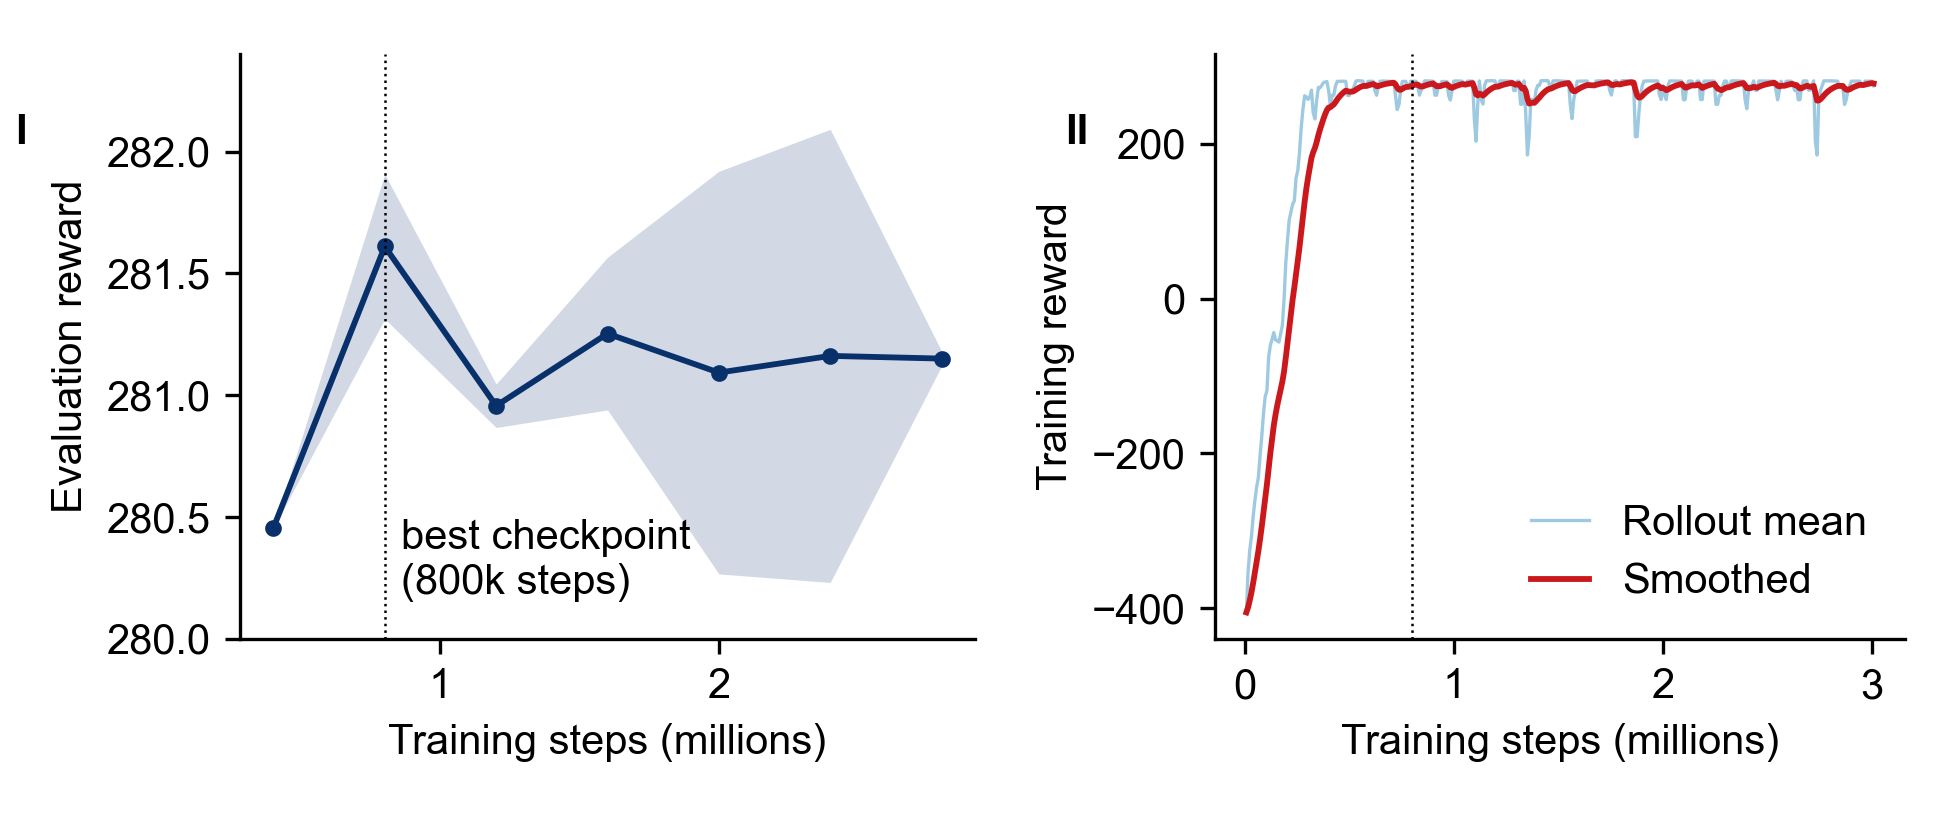
\includegraphics[width=0.82\linewidth]{fig6_learning.png}
  \caption{\textbf{Training performance and the checkpoint used for
    analysis.}
    \textbf{(Left panel)}~Evaluation reward across sampled checkpoints
    (mean $\pm$\,SD across evaluation episodes).
    \textbf{(Right panel)}~Per-episode training reward over the
    $3\times10^6$-step run (light blue) and its exponential moving average
    (red). All population and fixed-point analyses use the saved
    best-evaluation checkpoint, which corresponds to 800,000 training
    steps.}
  \label{fig:learning}
\end{figure}

\FloatBarrier

The best-evaluation checkpoint was saved at 800,000 steps and is the
checkpoint used for the reported rollouts and population analyses. A
separate fixed-point sensitivity analysis across eight saved checkpoints
showed appreciable variation in equilibrium locations and relaxation
times. The results should therefore be read as a characterization of this
selected policy, not as a checkpoint-invariant property of PPO training.

The clustering and decoding results in Figures~\ref{fig:pca}
and~\ref{fig:decoding} describe hidden-activity geometry. To examine local
physical stability, we analysed the policy--physics loop with forward
position and forward speed held fixed and the external impulse removed.
\label{sec:results-attractor}
The actor has no recurrent hidden state, so the fixed points are not
equilibria of hidden activity. We evaluated 280 episodes from the
best-evaluation checkpoint (800,000 training steps): 140 episodes per route,
with 20 episodes per condition on each route, from one training seed and
one evaluation seed. The force protocol is as specified in
Section~\ref{sec:methods-perturbation}; in particular, leftward magnitudes
were 0.40, 0.60, and 0.85, whereas rightward magnitudes were 0.40, 0.65,
and 1.80. The directions therefore do not provide matched-magnitude
comparisons. We solved for fixed points of the reduced lateral map
$(x,v_x)\mapsto(x_{t+1},v_{x,t+1})$ at $y=5.0$~m, separately for each
route cue, with forward speed fixed at its measured plateau and the
external force set to zero.
Both fixed points are locally stable, with two real eigenvalues below 1 in
magnitude and no imaginary component, so close to the fixed point the
lateral state relaxes back smoothly rather than oscillating.
The left-route fixed point sits at $x^{*}=3.321$~m with a relaxation time
constant of 1.42~s; the right-route fixed point sits at $x^{*}=6.705$~m
with a time constant of 1.34~s, close to a mirror image of the left about
the corridor midline at $x=5.0$~m.
Episodes that completed the detour crossed $y=5.0$~m at
$3.43\pm0.03$~m on the left route ($n=120$) and $6.62\pm0.05$~m on the
right route ($n=140$), which is 0.11~m and 0.09~m from the fixed points.
Across the eight saved checkpoints, fixed-point locations ranged from
3.23--3.62~m on the left route and 6.40--6.79~m on the right; relaxation
times ranged from 0.55--1.42~s and 0.76--1.34~s, respectively. The values
above therefore describe the selected checkpoint, not a checkpoint-
invariant property of training.

\begin{figure}[H]
  \centering
  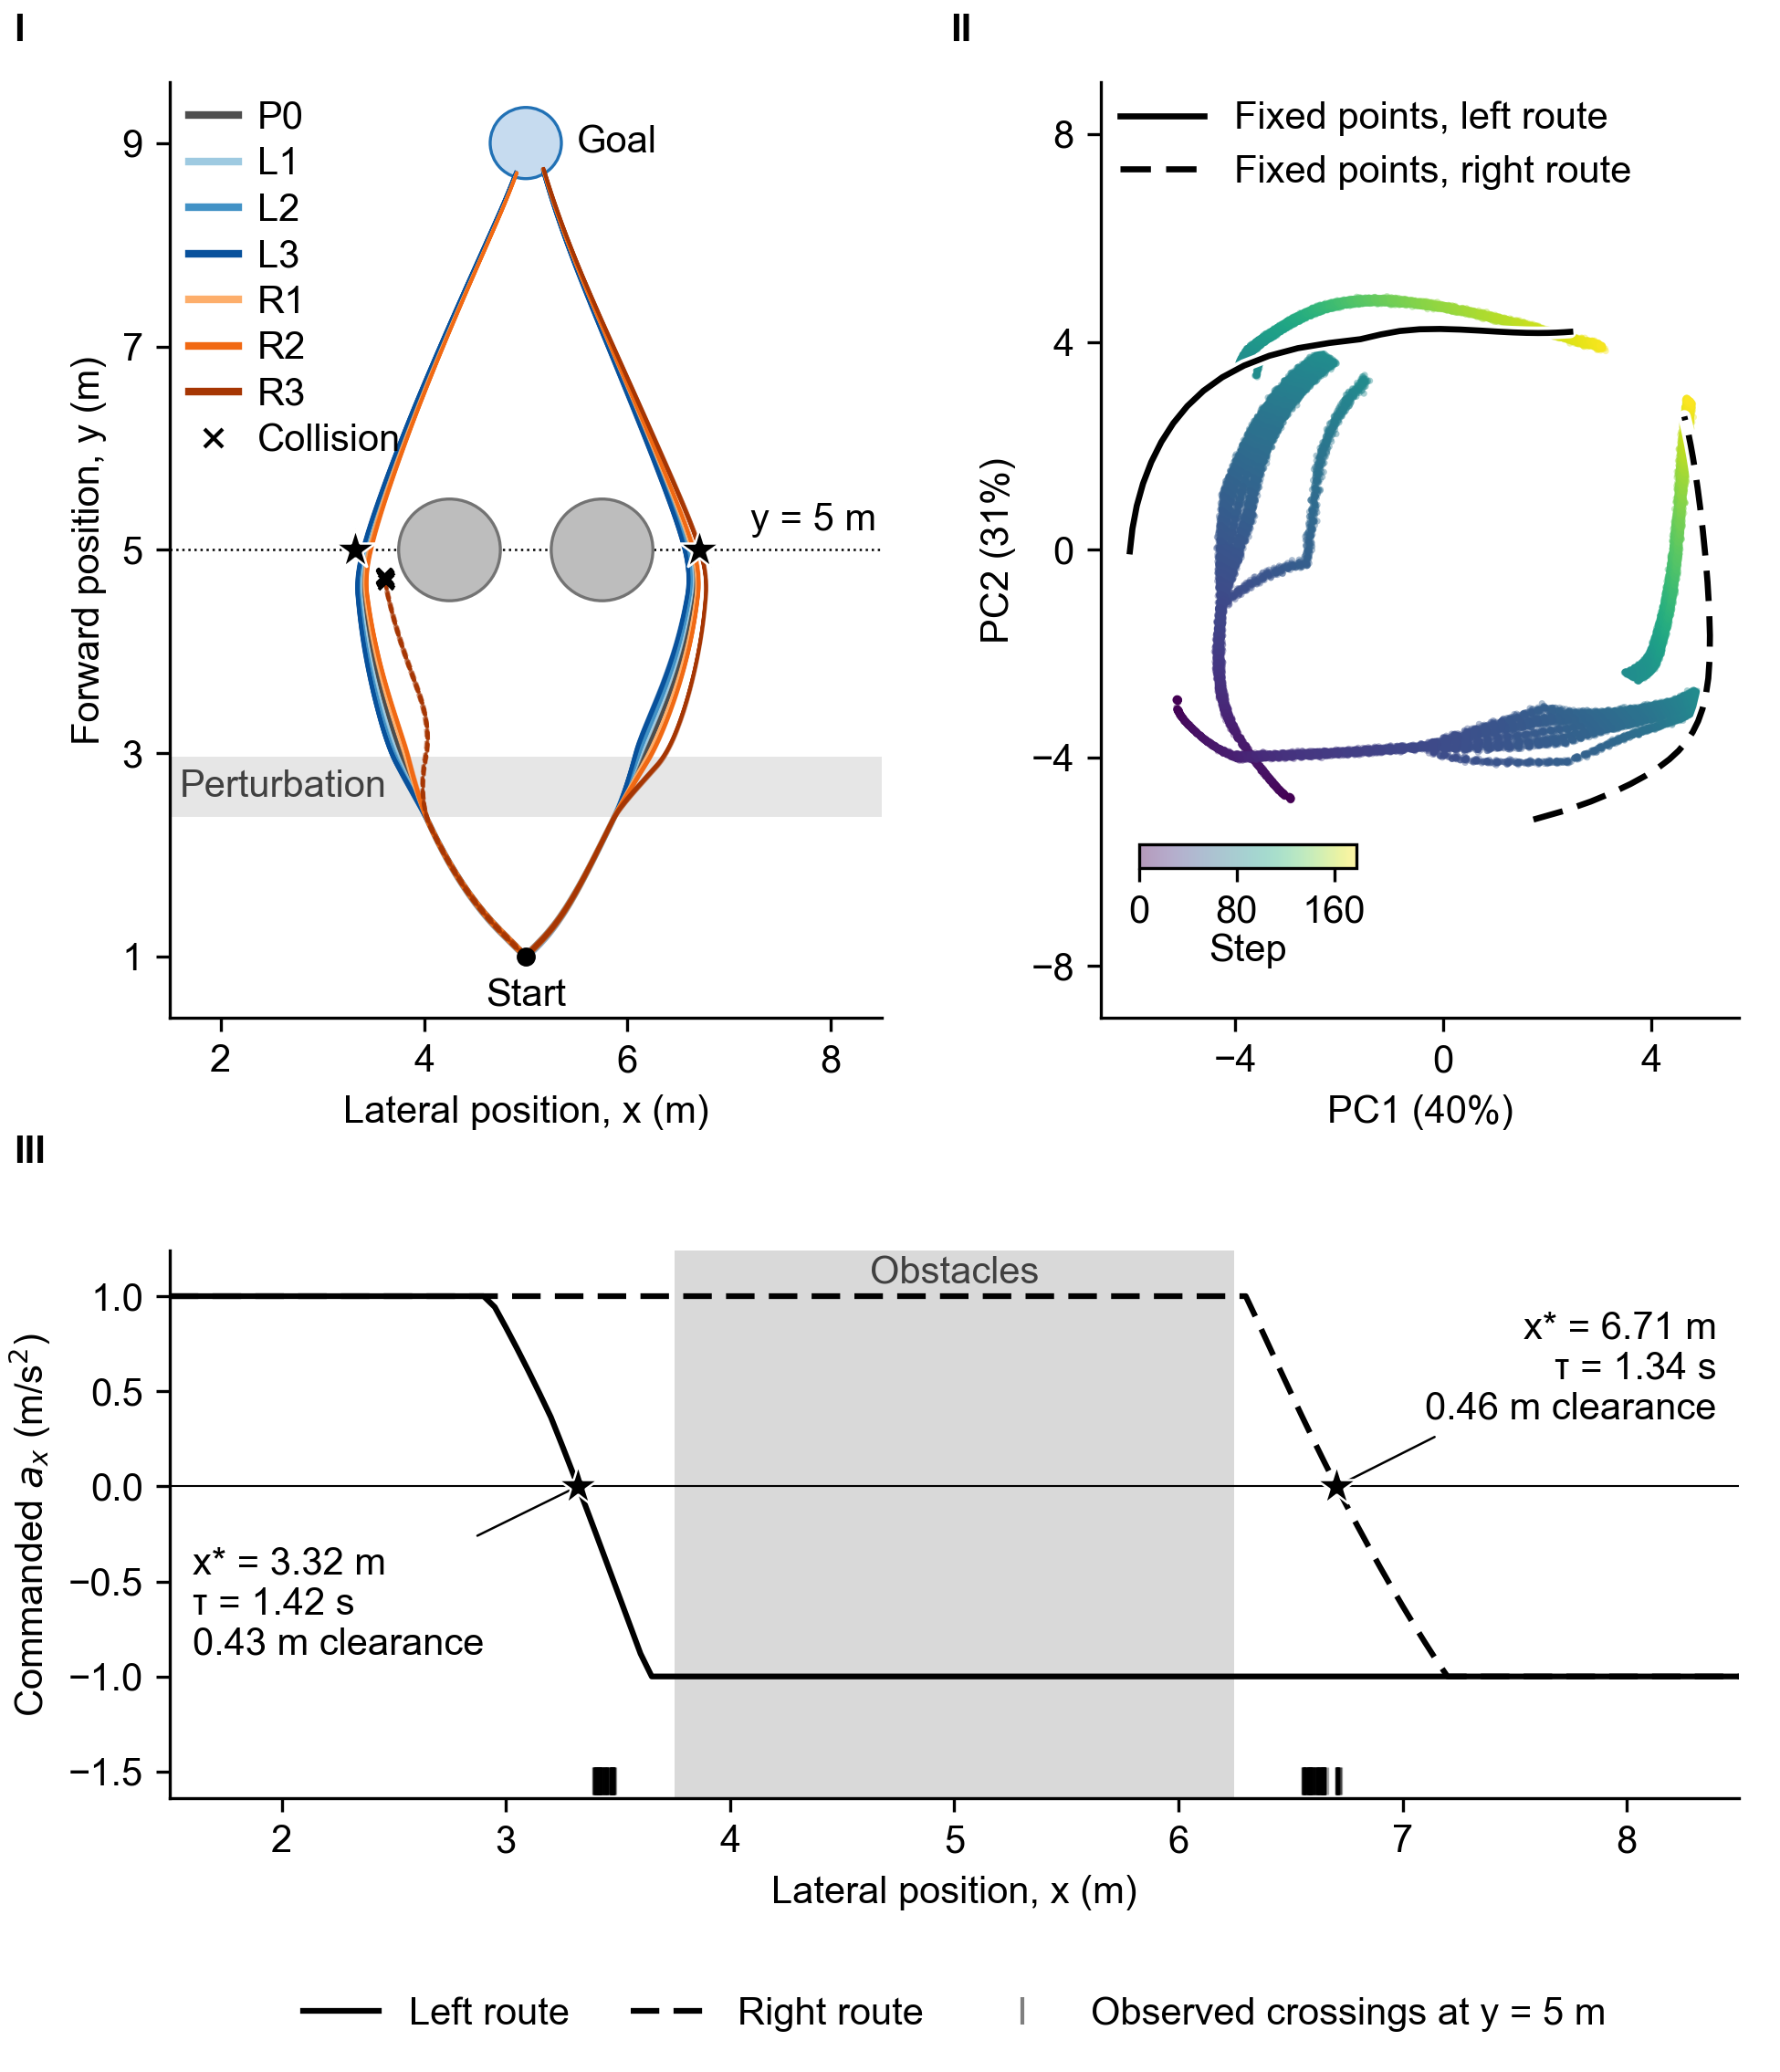
\includegraphics[width=0.95\linewidth]{figures/fig_composite_obstacle_avoidance_mechanism.png}
  \caption{\textbf{Reduced lateral fixed points, executed paths, and
    population activity in the policy--physics loop.}
    \textbf{(I)}~Reach trajectories for all seven conditions (colour) on
    both detour routes. Dashed lines and crosses mark collisions. The grey
    band is the span of heights at which the impulse acts (median over
    control episodes, steps 40--53). Stars mark the closed-loop fixed points
    at $y=5.0$~m.
    \textbf{(II)}~PC1--PC2 of hidden-layer activity from the same rollouts,
    coloured by step. The components are recomputed on these rollouts (70.6\%
    of variance in two components) so that the fixed-point states are
    projected through the same checkpoint that produced the activity. Black
    curves are the fixed-point states $x^{*}(y)$ for the left (solid) and
    right (dashed) route.
    \textbf{(III)}~Commanded lateral acceleration at $y=5.0$~m with
    $v_x=0$ and the forward speed at its plateau. Each route has one zero
    crossing with a negative slope, which is the fixed point. The commanded
    acceleration saturates at $\pm1$. Ticks along the bottom mark where
    completed episodes crossed $y=5.0$~m. Collisions occurred only for the
    largest tested rightward impulse on the left route (20 of 20 episodes).
    The plotted fixed-point curve is a set of local equilibria at fixed
    forward positions, not a trajectory that the agent follows exactly.}
  \label{fig:attractor}
\end{figure}

\FloatBarrier

The fixed points relate to the behavioural results locally, at the obstacle
band. The mean crossing position is within approximately 0.1~m of the
corresponding fixed point, but the equilibria do not track the complete
executed trajectory. Across $y=1.5$--$8.5$~m, the median absolute
fixed-point-to-mean-path difference was 0.63~m on the left route and
0.48~m on the right; the maximum differences were 1.67~m and 1.69~m.
This is consistent with a local stabilization interpretation at the sampled
forward position, not with a moving equilibrium that the reach follows
throughout.
Second, the fixed-point states lie within the region of recorded activity.
The median distance from a fixed-point state to the nearest recorded point in
PC1--PC2 is 0.35 units on the left route and 0.46 on the right, against 0.92
and 1.22 for states at random lateral positions at the same heights.
The largest distance along either curve is 1.6 units, so the curves are
close to the recorded activity but not on any one trajectory through it.
In these rollouts, a four-cluster partition of PC1--PC2 separates the two
routes as well as the phases, so it is not used here as a measure of phase.

The two fixed points are approximately symmetric in lateral position, but
the evaluation does not isolate the effect of force direction: the tested
rightward and leftward magnitudes are not matched, and the only observed
failure occurred for R3 on the left route. The data therefore do not
support a general claim that the controller is more vulnerable to one
direction, nor a prediction that vulnerability reverses on the other route.

%==============================================================
\section{Discussion}
%==============================================================

We asked how a reward-trained, memoryless controller responds to lateral
perturbations and whether its population activity and physical closed loop
offer complementary descriptions of that response. The analysed checkpoint
showed low-dimensional hidden activity, route-specific local lateral
equilibria, and post-impulse condition decodability. These findings are
descriptive and specific to one training run, checkpoint, and point-mass
task; they provide an organizational comparison with motor neuroscience,
not evidence of neural equivalence.

\paragraph{Behaviour and feedback correction.}

Across the 280 evaluation episodes, only one route-by-condition group
failed: all 20 left-route trials with the strongest tested rightward impulse
collided, while the corresponding right-route trials succeeded. The impulse
magnitudes were not matched across directions, so this result does not
establish a general directional asymmetry. It identifies a specific
failure mode of this checkpoint under this task geometry.

In biological reaching, unexpected forces evoke graded online corrections
that reshape the movement while progress toward the target continues
\citep{Pruszynski2012,Nashed2014,FlashHogan1985,Scott2004,Dimitriou2013,Shadmehr1994,Diedrichsen2010}.
The present model offers a simple setting in which to study how sensory
state, action, and physical feedback interact during such corrections.
However, a point mass controlled by a feedforward policy lacks muscle
mechanics, sensory noise, neural delays, and recurrent memory. Similarities
in behavioural organization therefore motivate comparison with biological
reaching; they do not establish shared neural mechanisms.

\paragraph{Population-state geometry.}

Two principal components explained 70.6\% of the variance in the analysed
256-unit layer. This describes the activity sampled in these rollouts; it
does not show that reinforcement learning alone created a neural-like
manifold. The task samples a restricted set of states, and the observation
includes an explicit route cue, both of which can contribute to the
low-dimensional structure. Motor-cortical reaching studies report
low-dimensional population activity
\citep{Churchland2012,Shenoy2013,Cunningham2014,Gallego2017}, providing an
organizational point of comparison rather than evidence of equivalence.

Exploratory $K$-means clustering with $K=4$ produced clusters ordered over
movement step within each route. The choice of $K$ was not cross-validated,
and these results come from one training seed. We regard the apparent
phase ordering as descriptive rather than evidence for discrete neural
states \citep{Churchland2012,Shenoy2013,Kaufman2014,Elsayed2016,Georgopoulos1986}.

\paragraph{What the decoder tells us about internal organisation.}

The episode-held-out decoder distinguished perturbation condition after
the impulse, but not before it. This is state decoding, not evidence that a
memoryless policy stores perturbation history or causally uses a decoded
signal. The actor receives current kinematics and task context, so a
changed physical state is sufficient to make conditions distinguishable.
This distinction also matters when interpreting decoders of
motor-cortical activity: condition information should be tested after
accounting for movement state, and decoding alone does not establish the
role of that information in generating a correction
\citep{Nashed2014,Churchland2012,Sadtler2014,Perich2018}.
A useful next comparison would condition neural decoding on hand state and
contrast single-time-point with temporally integrated activity.

\paragraph{Limitations.}

Several constraints bound the generality of these conclusions.

\textit{Single training seed.}
All results are from one PPO training run and its best-evaluation
checkpoint at 800,000 steps. Across eight saved checkpoints, the lateral
fixed-point locations and relaxation times varied appreciably. Multi-seed
and checkpoint analyses are needed to establish which aspects of the
activity geometry and closed-loop stability are reliable properties of
the task and learning procedure.

\textit{Simplified environment and feedforward policy.}
The two-dimensional point-mass environment omits limb and muscle mechanics,
sensory noise, and neural delays. The feedforward actor processes each
observation independently and cannot explicitly maintain a temporal
estimate of a perturbation. These choices make the policy--physics loop
tractable to analyse, but limit the biological claims and the range of
corrections the model can represent.

\textit{Descriptive analyses.}
PCA, clustering, and linear decoding describe structure but do not
identify which hidden units cause behaviour. Likewise, a locally stable
fixed point does not by itself show that perturbation recovery is caused
by attraction to that point. Causal interventions and matched-force
experiments are needed to test these mechanisms.

\textit{Use of AI tools.}
Large language models were used to support text editing, proofreading,
debugging, and \LaTeX\ formatting.

\paragraph{Connecting to biological motor systems.}

These results do not show that an artificial hidden layer reproduces motor
cortex. They show that a relatively simple, feedforward controller can
exhibit low-dimensional activity and route-specific local stability when
coupled to physical feedback. This makes it a tractable reference for
asking which features of population activity arise from task structure,
which reflect the policy, and which depend on the dynamics of the body and
environment \citep{Churchland2012,Gallego2017,Oby2019,Crevecoeur2019}.
For neuroscience, a useful next step is to compare matched perturbations
across route plans while measuring both movement and population activity,
and to ask whether condition decoding persists after accounting for hand
state. For assistive control, the same analyses may eventually help relate
controller state to failure risk, but that application remains to be
tested in richer dynamics and across multiple policies.

%==============================================================
\section{Conclusion}
%==============================================================

We trained a PPO controller for obstacle avoidance, tested it with
seven lateral-force conditions, and analysed one hidden layer alongside
the controller--physics loop. Two principal components explained 70.6\%
of activity variance, while an episode-held-out decoder identified
perturbation condition after, but not before, the impulse. At the obstacle
band, the reduced lateral dynamics had a locally stable fixed point for
each route cue. These are properties of one feedforward policy and one
point-mass task, not evidence that artificial units reproduce neural
activity.

The behavioral record is also specific: the strongest tested rightward
impulse caused collisions on the left route, while all other
route-by-condition groups succeeded. Since the leftward and rightward
impulse magnitudes were not matched, we cannot attribute that outcome to
direction alone. The fixed points describe local lateral stability at a
fixed forward position; they do not explain the entire reach or establish
that the executed trajectory follows a moving equilibrium.

By linking perturbation outcomes to measurable local properties of the
policy--environment loop, this simple model offers a testable reference for
asking how feedback helps biological motor systems preserve goal-directed
action under perturbation, and a starting point for more reliable assistive
controllers.

%==============================================================
\section*{Acknowledgments}
%==============================================================

This work was supported in part by the Connected Minds Program,
Canada First Research Excellence Fund,
Grant No.~CFREF-2022-00010.

\bibliographystyle{unsrtnat}
\bibliography{references}

\end{document}
